\section{Aszinkron üzenetsor}

A service felelőssége, hogy az egyes elvégzendő feladatokat ütemezze,
és azok a megfelelő feldolgozóegységekhez eljuttassa.

A működés során fontos, hogy az üzenetek ne vesszenek el (pl. ha a
szolgáltatás újraindul), ehhez szükség van a megfelelő kommunikációs és
tranzakciós protokollokra. Mivel ezek megvalósítása a gyakorlatban sok
körültekintést igényel, így elvetettem a saját megoldás implementálásának
lehetőségét.

A RabbitMQ szoftvert választottam a feladatra, ami az AMQP specifikációt
implementáló Erlang-alapú szoftver. Az egyes szoftverkomponensek egy RabbitMQ
szerveren keresztül kommunikálnak, így ha egy szolgáltatás rövid időre leáll,
akkor a függőben lévő üzenetek a szerveren tárolódnak (természetesen itt is
perzisztensen, így a RabbitMQ szerver leállása vagy meghibásodása esetén sem
kell tartani az adatvesztéstől).

A szerver feladata elsősorban az üzenetek továbbítása, azonban az üzenetsor
működésének jellegét kihasználva egy \emph{resource pool}-t is megvalósítottam
vele. Az egyes feladatok elvégzéséhez szükség van \emph{tokenekre}, melyek
segítségével autentikált Twitter API hívások végezhetők, mivel azonban ezek
használata erősen korlátozott (adott időintervallumban csak bizonyos számú
API hívás végezhető el), így meg kell akadályozni, hogy az egyes tokenek
``kimerüljenek'', azaz kölcsönös kizárást kell biztosítani hozzájuk,
azokat csak meghatározott időközönként lehet újra felhasználni.
A vázlatos működés \aref{fig:queue}. ábrán látható.

\begin{figure}[h!]
  \centering
  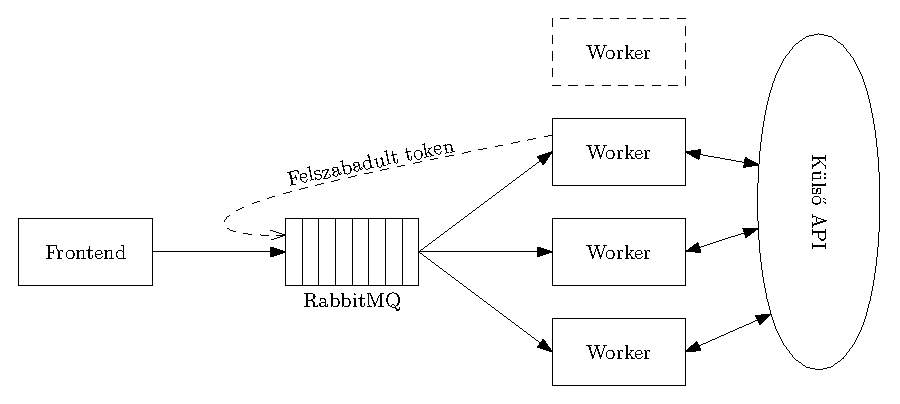
\includegraphics[width=0.95\textwidth]{figures/queue}
  \caption{Az üzenetsor szerepe az alkalmazásban}
  \label{fig:queue}
\end{figure}

\subsection{AMQP}

Az AMQP (Advanced Message Queuing Protocol) egy rugalmas protokoll üzenetek
változatos minták szerinti továbbítására. A \emph{termelők} a szerverhez
kapcsolódva egy \emph{exchange}-ben publikálják az üzenetüket,
a szerver pedig az üzenet \emph{routing key}-e
(és az aktuális \emph{exchange-queue bindingok}) alapján továbbítja a
megfelelő \emph{queue(k)}-ba. A \emph{fogyasztók} az egyes queue-kra
iratkoznak fel, a szerver pedig továbbítja az üzenetet egy (vagy több)
fogyasztónak.

Az elkészült alkalmazás nem használ bonyolult mintákat, minden üzenet
az alapértelmezett exchangen keresztül publikálódik, a routing key pedig
megegyezik a queue nevével, ami pedig az adott feladat nevével egyezik meg,
így az egyszerűség kedvéért a továbbiakban az üzenet publikálás alatt
azt lehet érteni, hogy megérkezik a routing key-nek megfelelő queue-ba az
üzenet.

\subsection{Resource pool}

Az egyes tokenek felhasználása korlátozott, így a befejezett feladat után
nem szabad azt rögtön visszarakni a pool-ba, hanem bizonyos ideig
``várakoztatni'' kell.

Ezt egy közbenső queue beiktatásával oldom meg. Az AMQP protokol támogatja,
hogy az egyes üzenetekhez TTL-t (Time to Live) rendeljünk.
Ha az üzenetet nem sikerült ezen idő alatt eljuttatni egy fogyasztóhoz,
akkor automatikusan \emph{dead} állapotú lesz. Ha a queue-nak beállítunk
ún. \emph{dead-letter-exchange}-t, akkor ezek az üzenetek kiürülnek az
üzenetsorból, és újra publikálódnak a megadott exchange-n, a megadott
routing key-el (\emph{dead-letter-routing-key}).

Ezt kihasználva, használat után az egyes tokenek egy olyan queue-ba kerülnek,
aminek nincsenek fogyasztói, ezért a megfelelő idő eltelte után újra
visszakerülnek a pool-ba. A működés \aref{fig:pool}. ábrán látható.

\begin{figure}[h!]
  \centering
  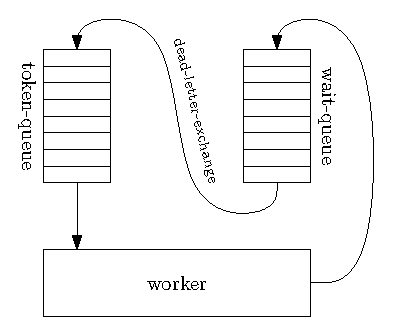
\includegraphics[width=0.6\textwidth]{figures/pool}
  \caption{Resource pool megoldás}
  \label{fig:pool}
\end{figure}

Mivel a TTL a queue-ra nézve állandó (létezik az üzenetre értelmezett TTL is,
de az nem használható az általam elérni kívánt funkcionalitáshoz), így
minden TTL-hez külön queue-t kell deklarálni.
Erre hoztam létre az \verb=amqp-schedule= modult. A könyvtár egy egyszerű
interfésszel elrejti előlünk ezt az ideiglenes üzenetsort:

\begin{js}
  var scheduler = require('amqp-schedule');
  var publish = scheduler(conn); // conn: amqp kliens objektum

  publish(exchange, key, message, delay, opts, cb);
  // vagy
  publish(exchange, key, message, date, opts, cb);
\end{js}

A késleltetés a \verb=delay= paraméterrel szabályozható, vagy konkrét időpont
(\verb=date=) is megadható. A háttérben egy speciálisan elnevezett
queue jön létre, ami a megfelelő \emph{dead-letter-exchange},
\emph{dead-letter-routing-key} és \emph{message-ttl} paraméterekkel rendelkezik,
azaz a megadott idő után az üzenet automatikusan a cél queue-ba kerül.
Mivel az eltérő időzítések új üzenetsorokat hoznak létre, így
a létrejött ideiglenes queue-k rendelkeznek \emph{expires} paraméterrel,
ami azt szabja meg, hogy mennyi \emph{idle} idő (üresjáratban töltött)
után szűnjenek meg maguktól. Így a szerver védve van attól, hogy a már nem
használt, üres üzenetsorok erőforrásokat foglaljanak.
